
% generated with https://www.mathcha.io/editor

\tikzset{every picture/.style={line width=0.75pt}} %set default line width to 0.75pt        

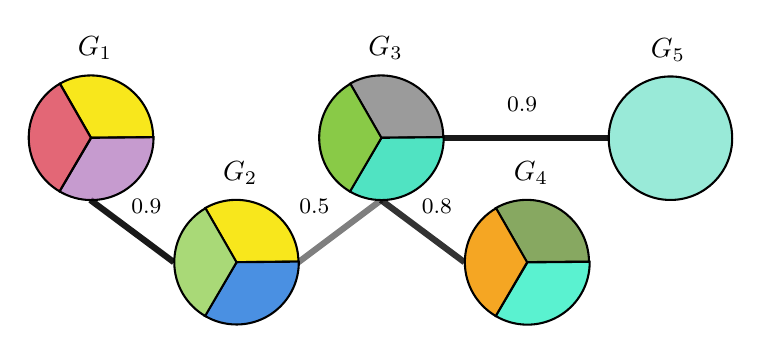
\begin{tikzpicture}[x=0.75pt,y=0.75pt,yscale=-1,xscale=1]
%uncomment if require: \path (0,1438); %set diagram left start at 0, and has height of 1438

%Straight Lines [id:da05066971896839911] 
\draw [color={rgb, 255:red, 0; green, 0; blue, 0 }  ,draw opacity=0.9 ][line width=2.25]    (189.75,629.92) -- (230,659.92) ;
%Straight Lines [id:da2380834376560974] 
\draw [color={rgb, 255:red, 0; green, 0; blue, 0 }  ,draw opacity=0.5 ][line width=2.25]    (290,659.92) -- (330,629.92) ;
%Straight Lines [id:da5855553922835157] 
\draw [color={rgb, 255:red, 0; green, 0; blue, 0 }  ,draw opacity=0.8 ][line width=2.25]    (329.75,629.92) -- (370,659.92) ;
%Straight Lines [id:da25734644353540226] 
\draw [color={rgb, 255:red, 0; green, 0; blue, 0 }  ,draw opacity=0.9 ][line width=2.25]    (359.5,600.17) -- (439.5,600.17) ;
%Shape: Pie [id:dp628461760630195] 
\draw  [fill={rgb, 255:red, 248; green, 231; blue, 28 }  ,fill opacity=1 ] (175.1,573.88) .. controls (179.49,571.36) and (184.58,569.92) .. (190,569.92) .. controls (206.48,569.92) and (219.86,583.21) .. (220,599.65) -- (190,599.92) -- cycle ;
%Shape: Pie [id:dp9417219236919072] 
\draw  [fill={rgb, 255:red, 170; green, 106; blue, 183 }  ,fill opacity=0.67 ] (220.19,599.67) .. controls (220.19,599.77) and (220.19,599.87) .. (220.19,599.97) .. controls (220.19,616.53) and (206.76,629.97) .. (190.19,629.97) .. controls (184.62,629.97) and (179.39,628.44) .. (174.92,625.79) -- (190.19,599.97) -- cycle ;
%Shape: Pie [id:dp9576808981889051] 
\draw  [fill={rgb, 255:red, 208; green, 2; blue, 27 }  ,fill opacity=0.6 ] (174.92,625.79) .. controls (166.03,620.59) and (160.06,610.93) .. (160.06,599.89) .. controls (160.06,588.77) and (166.11,579.06) .. (175.1,573.88) -- (190.06,599.89) -- cycle ;
%Shape: Pie [id:dp0633105132933407] 
\draw  [fill={rgb, 255:red, 155; green, 155; blue, 155 }  ,fill opacity=1 ] (314.9,573.88) .. controls (319.29,571.36) and (324.38,569.92) .. (329.81,569.92) .. controls (346.29,569.92) and (359.66,583.21) .. (359.8,599.65) -- (329.81,599.92) -- cycle ;
%Shape: Pie [id:dp5227249119465338] 
\draw  [fill={rgb, 255:red, 80; green, 227; blue, 194 }  ,fill opacity=1 ] (360,599.67) .. controls (360,599.77) and (360,599.87) .. (360,599.97) .. controls (360,616.53) and (346.57,629.97) .. (330,629.97) .. controls (324.42,629.97) and (319.2,628.44) .. (314.73,625.79) -- (330,599.97) -- cycle ;
%Shape: Pie [id:dp24565430499054774] 
\draw  [fill={rgb, 255:red, 137; green, 202; blue, 71 }  ,fill opacity=1 ] (314.86,625.87) .. controls (305.97,620.67) and (300,611.01) .. (300,599.97) .. controls (300,588.85) and (306.05,579.14) .. (315.04,573.96) -- (330,599.97) -- cycle ;
%Shape: Pie [id:dp5392854442993551] 
\draw  [fill={rgb, 255:red, 65; green, 117; blue, 5 }  ,fill opacity=0.63 ] (385.1,633.83) .. controls (389.49,631.31) and (394.58,629.87) .. (400,629.87) .. controls (416.48,629.87) and (429.86,643.16) .. (430,659.61) -- (400,659.87) -- cycle ;
%Shape: Pie [id:dp26888536672116814] 
\draw  [fill={rgb, 255:red, 90; green, 242; blue, 208 }  ,fill opacity=1 ] (430.33,659.71) .. controls (430.33,659.8) and (430.33,659.9) .. (430.33,660) .. controls (430.33,676.57) and (416.9,690) .. (400.33,690) .. controls (394.75,690) and (389.53,688.48) .. (385.06,685.83) -- (400.33,660) -- cycle ;
%Shape: Pie [id:dp6741062860408691] 
\draw  [fill={rgb, 255:red, 245; green, 166; blue, 35 }  ,fill opacity=1 ] (385.06,685.83) .. controls (376.17,680.62) and (370.19,670.97) .. (370.19,659.92) .. controls (370.19,648.8) and (376.24,639.09) .. (385.23,633.91) -- (400.19,659.92) -- cycle ;
%Shape: Pie [id:dp2675319000886982] 
\draw  [fill={rgb, 255:red, 248; green, 231; blue, 28 }  ,fill opacity=1 ] (245.1,633.83) .. controls (249.49,631.31) and (254.58,629.87) .. (260,629.87) .. controls (276.48,629.87) and (289.86,643.16) .. (290,659.61) -- (260,659.87) -- cycle ;
%Shape: Pie [id:dp5836494702687516] 
\draw  [fill={rgb, 255:red, 74; green, 144; blue, 226 }  ,fill opacity=1 ] (290.19,659.63) .. controls (290.19,659.72) and (290.19,659.82) .. (290.19,659.92) .. controls (290.19,676.49) and (276.76,689.92) .. (260.19,689.92) .. controls (254.62,689.92) and (249.39,688.4) .. (244.92,685.75) -- (260.19,659.92) -- cycle ;
%Shape: Pie [id:dp49334724962429766] 
\draw  [fill={rgb, 255:red, 169; green, 217; blue, 119 }  ,fill opacity=1 ] (245.06,685.83) .. controls (236.17,680.62) and (230.19,670.97) .. (230.19,659.92) .. controls (230.19,648.8) and (236.24,639.09) .. (245.23,633.91) -- (260.19,659.92) -- cycle ;
%Shape: Circle [id:dp7055246821331733] 
\draw  [fill={rgb, 255:red, 153; green, 234; blue, 216 }  ,fill opacity=1 ] (439.5,600.17) .. controls (439.5,583.74) and (452.82,570.42) .. (469.25,570.42) .. controls (485.68,570.42) and (499,583.74) .. (499,600.17) .. controls (499,616.6) and (485.68,629.92) .. (469.25,629.92) .. controls (452.82,629.92) and (439.5,616.6) .. (439.5,600.17) -- cycle ;

% Text Node
\draw (192,556.92) node   [align=left] {$\displaystyle G_{1}$};
% Text Node
\draw (262,616.92) node   [align=left] {$\displaystyle G_{2}$};
% Text Node
\draw (332,556.92) node   [align=left] {$\displaystyle G_{3}$};
% Text Node
\draw (402,616.92) node   [align=left] {$\displaystyle G_{4}$};
% Text Node
\draw (468,557.5) node   [align=left] {$\displaystyle G_{5}$};
% Text Node
\draw (289,628) node [anchor=north west][inner sep=0.75pt]   [align=left] {{\footnotesize 0.5}};
% Text Node
\draw (208,628) node [anchor=north west][inner sep=0.75pt]   [align=left] {{\footnotesize 0.9}};
% Text Node
\draw (389,579) node [anchor=north west][inner sep=0.75pt]   [align=left] {{\footnotesize 0.9}};
% Text Node
\draw (348,628) node [anchor=north west][inner sep=0.75pt]   [align=left] {{\footnotesize 0.8}};


\end{tikzpicture}
